\documentclass[a4paper,12pt]{article}
\usepackage[english]{babel}
\usepackage[utf8]{inputenc}
\usepackage{graphicx}

%
% For alternative styles, see the biblatex manual:
% http://mirrors.ctan.org/macros/latex/contrib/biblatex/doc/biblatex.pdf
%
% The 'verbose' family of styles produces full citations in footnotes, 
% with and a variety of options for ibidem abbreviations.
%
\usepackage{csquotes}
\usepackage[style=verbose-ibid,backend=bibtex]{biblatex}
\bibliography{sample}

\usepackage{enumitem} % for customizing lists
\usepackage{amsmath} 

\title{WU-E model Verification Technical Guide}

\author{writeLaTeX}

\date{\today}

\begin{document}
\maketitle

This document lays out the governing equations and definitions behind the MATLAB prototype for the WU--E (urban structure) heat-flux model with an anisotropic (wind-aligned) fire ellipse and a piecewise transient HRR curve.

\section{Symbols, Defaults, and Units}

\noindent\textbf{Given (defaults in brackets):}
\begin{itemize}[leftmargin=1.5em]
  \item Non-burnable fraction of structure: $\mathrm{NONBURNABLE\_FRAC}$ [0]
  \item Effective absorptivity for radiation: $\alpha$ (= \texttt{ABSORPTIVITY}) [0.89]
  \item Radiation cut-off distance (m): $R_{\mathrm{rad}}$ (= \texttt{RAD\_DIST}) [100\,m]
  \item Analysis cell size (m): $\Delta$ (= \texttt{ANALYSIS\_CELLSIZE}) [20\,m]
  \item Wind direction (deg, meteorological, blowing \emph{from}): $\mathrm{WD_{20ft}}$ [0$^\circ$]
  \item Wind speed at 20 ft (mph): $\mathrm{WS_{20ft}}$ [40\,mph]
  \item Average footprint dimension (m): $A$ (= \texttt{HAMADA\_A}) [10\,m]
  \item Average separation distance (m): $D$ (= \texttt{HAMADA\_D}) [10\,m]
  \item Wind proportionality factor (--): $W_p$ (= \texttt{WIND\_PROP}) [1]
\end{itemize}

\noindent\textbf{Design fire curve parameters:}
\begin{itemize}[leftmargin=1.5em]
  \item Early/developing time: $t_{\mathrm{early}}$ [300 s]
  \item Fully developed (plateau) end time: $t_{\mathrm{dev}}$ [3900 s]
  \item Decay end time: $t_{\mathrm{decay}}$ [4200 s]
  \item Peak heat release rate per unit area: $\mathrm{HRRPUA_{peak}}$ [400\,kW/m$^2$]
\end{itemize}

\noindent\textbf{Index grid:} integer indices $i,j\in\{-5,\ldots,5\}$ with centers located at $(x,y)=(i\,\Delta,\; j\,\Delta)$ relative to the burning structure at the origin $(0,0)$.

\section{Coordinate Transformations (need clarify)}

Let the geometric angle from source to target be
\begin{equation}
  \theta=\arctan(j,\; i)\quad \text{(radians)}.
\end{equation}
Wind-aligned major-axis angle (radians) is
\begin{equation}
  \theta_{\mathrm{wind}}=\frac{\pi}{180}\,(270-\mathrm{WD_{20ft}})\, .
\end{equation}
The relative angle (between major axis and line segment between source and target) used by the ellipse formulas is
\begin{equation}
  \theta_f=\theta-\theta_{\mathrm{wind}}\, .
\end{equation}
The radial distance from the source to the target cell center is
\begin{equation}
  R=\sqrt{(i\,\Delta)^2+(j\,\Delta)^2}\, .
\end{equation}

\begin{figure}[h!]
	\centering
	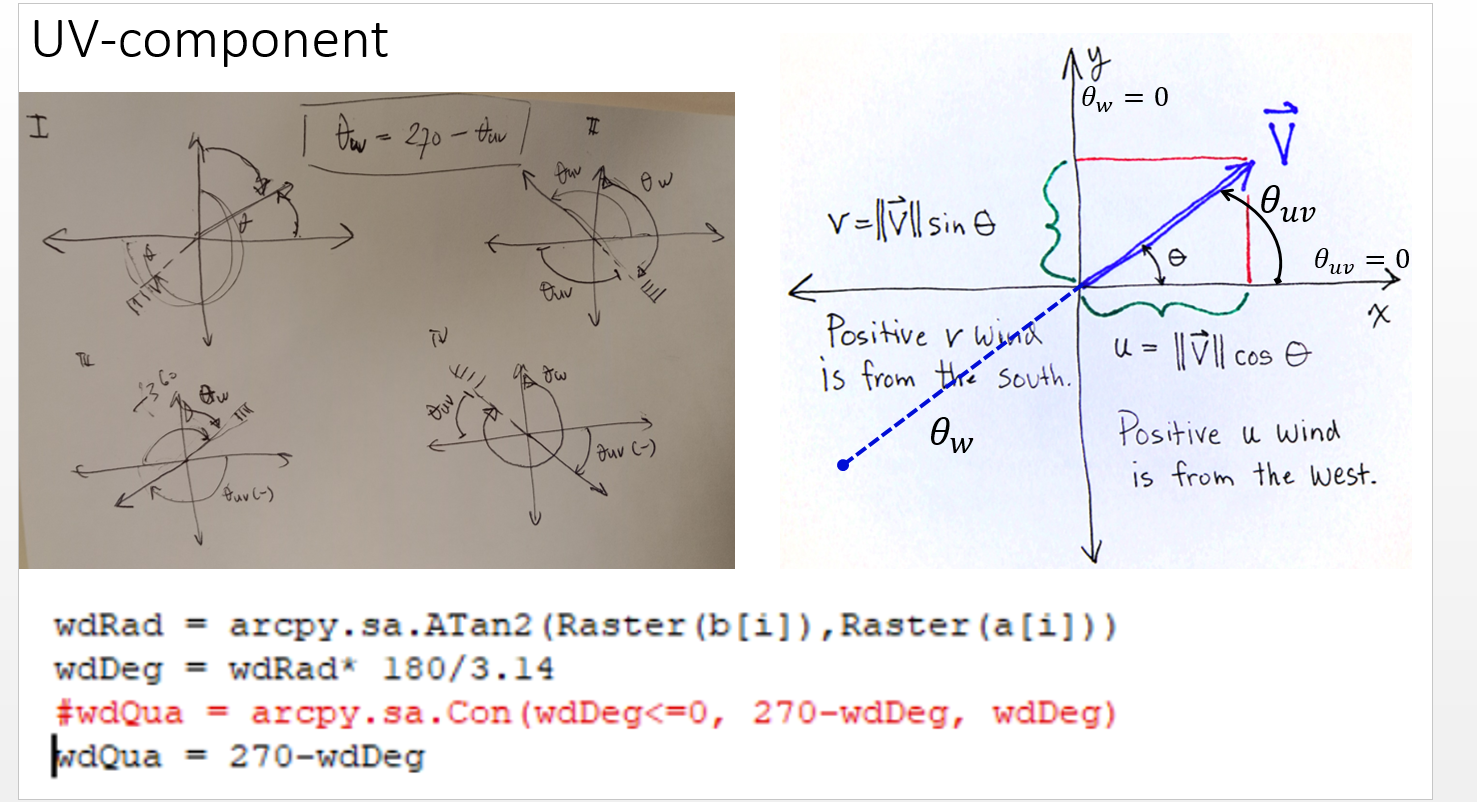
\includegraphics[width=\textwidth]{Figs/degTransformation.png}
	\caption{Explanation on the clarification}
	\label{fig:models_and_rules}
\end{figure}

\section{Wind-Aligned Ellipse (Hamada-style Regression)}\label{ellipse}

Convert wind speed to m/s:
\begin{equation}
  V=0.447\,\mathrm{WS_{20ft}}\, .
\end{equation}
The downwind ($D_\downarrow$), upwind ($D_\uparrow$), and sidewind ($D_\perp$) distances (m) are obtained by piecewise regressions in $V$ with linear or quadratic forms, parameterized by $(A,D)$, and scaled by $W_p$.

\subsection*{Low wind: $V<10\,\mathrm{m\,s^{-1}}$}
\begin{align}
D_\downarrow &= W_p\,(D_1 V + D_2)\\
D_\perp &= W_p\,(S_1 V + S_2)\\
D_\uparrow &= W_p\,(U_1 V + U_2)
\end{align}

\begin{align}
D_1&=1.679463256-0.123901243\cdot A+0.307612446\cdot D \nonumber\\
D_2&=78.62957398+1.536189561\cdot A-0.5662073\cdot D \nonumber\\
S_1&=-2.922896622-0.05550541\cdot A+0.017291361\cdot D \nonumber\\
S_2&=39.31478699+0.768094781\cdot A-0.28310365\cdot D \nonumber\\
U_1&=-6.297892493-0.119654483\cdot A+0.037754535\cdot D \nonumber\\
U_2&=78.62957398+1.536189561\cdot A-0.5662073\cdot D \nonumber
\end{align}

\subsection*{High wind: $V>17.3\,\mathrm{m\,s^{-1}}$}
\begin{align}
D_\downarrow &= W_p\,(D_1 V + D_2)\\
D_\perp &= W_p\,(S_1 V + S_2)\\
D_\uparrow &= W_p\,(U_1 V + U_2)
\end{align}

\begin{align}
D_1&=-7.159031537-0.043555289\cdot A-0.14894238\cdot D,\nonumber\\ D_2&=394.4930697+0.720929023\cdot A+11.42149084\cdot D,\nonumber\\
S_1&=-0.577270631-0.015285438\cdot A+0.012786629\cdot D,\nonumber\\
S_2&=38.11784939+0.800599307\cdot A-0.412476476\cdot D,\nonumber\\
U_1&=-1.092711783-0.025390239\cdot A+0.016740663\cdot D,\nonumber\\
U_2&=52.39584604+1.104793131\cdot A-0.57241037\cdot D.\nonumber
\end{align}

\subsection*{Moderate wind: $10\le V\le 17.3\,\mathrm{m\,s^{-1}}$}
\begin{align}
D_\downarrow &= W_p\,(D_1 V^2 + D_2 V + D_3)\\
D_\perp &= W_p\,(S_1 V^2 + S_2 V + S_3)\\
D_\uparrow &= W_p\,(U_1 V^2 + U_2 V + U_3)
\end{align}

\begin{align}
D_1&=4.099488028-0.000767118\cdot A+0.134372426\cdot D,\nonumber\\
D_2&=-94.26651508-0.000694022\cdot A-3.053034015\cdot D,\nonumber\\ D_3&=615.192675+0.300438559\cdot A+19.34120221\cdot D,\nonumber\\
S_1&=0.437844987+0.008280661\cdot A-0.002833081\cdot D,\nonumber\\
S_2&=-10.13978982-0.192922421\cdot A+0.067862023\cdot D,\nonumber\\
S_3&=66.32382799+1.282260348\cdot A-0.484673257\cdot D,\nonumber\\
U_1&=0.525004045+0.01046073\cdot A-0.004473105\cdot D,\nonumber\\
U_2&=-12.4091466-0.249326233\cdot A+0.109759448\cdot D,\nonumber\\
U_3&=84.64808209+1.727651884\cdot A-0.801945211\cdot D\nonumber
\end{align}

\subsection*{Ellipse parameters (need clarify)}

Major-axis semi-distance and eccentricity surrogate:
\begin{align}
a &= \frac{D_\downarrow + D_\uparrow}{2},\\
\varepsilon &= \min\!\Big(\tfrac{a}{2},\; a-D_\uparrow\Big).
\end{align}
Define
\begin{equation}
E_{b2}=1-\Big(\tfrac{\varepsilon}{a}\Big)^2\, .
\end{equation}
Then the minor axis is
\begin{equation}
b=\begin{cases}
\dfrac{D_\perp}{\sqrt{E_{b2}}}, & E_{b2}>0,\\[6pt]
0,& E_{b2}\le 0.
\end{cases}
\end{equation}
We also carry $D_\downarrow$ forward for downstream distance limiting.

\noindent\textbf{Ellipse state vector:}
\begin{equation}
\mathbf{E}=[\,a,\;b,\;\varepsilon,\;D_\downarrow\,]^{\mathsf T}.
\end{equation}

\section{Direct Flame Contact/Radiation Coverage  (need clarify, better with a schematic)} \label{heat_flux_calc_1}

The maximum ellipse reach (scalar, m) (what is the 0.3?):
\begin{equation}
R_{\max}=0.3\,D_\downarrow\,\frac{a-\varepsilon}{b^2}\, .
\end{equation}
Directional reach along angle $\theta_f$:
\begin{equation}
R_{\mathrm{ell}}(\theta_f)=\frac{R_{\max}\,b^2}{a-\varepsilon\,\cos\theta_f}\, .
\end{equation}
\textbf{DFC cell-coverage fraction} (clipped to $[0,1]$):
\begin{equation}
C_{\mathrm{DFC}}=\max\left[\min\left(\frac{R_{\mathrm{ell}}(\theta_f)+\tfrac{1}{2}\Delta - R}{\Delta},\,1\right),\,0\right].
\end{equation}
\textbf{Radiation coverage fraction} (annulus outside DFC, within cutoff):
\begin{align}
R_{\mathrm{rad\,limit}}(\theta_f)&=R_{\mathrm{ell}}(\theta_f)+R_{\mathrm{rad}},\\[4pt]
\Delta_{\mathrm{rad}}&=\max\left[\min\left(\frac{R_{\mathrm{rad\,limit}}(\theta_f)+\tfrac{1}{2}\Delta - R}{\Delta},\,0\right),\,1\right],\\[4pt]
F_{\mathrm{rad}}&=\Delta_{\mathrm{rad}}\bigl(1-C_{\mathrm{DFC}}\bigr). (why?)
\end{align}

\section{HRR Normalization over the Ellipse (Per-Cell Adjuster)}

Let the per-cell area be $\Delta^2$. To conserve total HRRPUA over the ellipse footprint, use
\begin{equation}
C_\mathrm{HRR}=\frac{\Delta^2}{\pi\,\left(\frac{b}{a}\right)\,a\,b}=\frac{\Delta^2}{\pi\,b^2}\, .
\end{equation}
(The implemented form uses $C_\mathrm{HRR}=\dfrac{\Delta^2}{\pi\,\mathrm{C_{adj}}\,a\,b}$ with $\mathrm{C_{adj}}=b/a$, which simplifies to the same expression.) (where does the $\mathrm{C_{adj}}=b/a$ come from?)

\section{Transient HRRPUA (Design Fire Curve)}\label{hrrpua}

For burning time $\tau$ and parameters $(t_{\mathrm{early}}, t_{\mathrm{dev}}, t_{\mathrm{decay}}, \mathrm{HRRPUA_{peak}})$:
\begin{equation}
\mathrm{HRRPUA}(\tau)=
\begin{cases}
\dfrac{\mathrm{HRRPUA_{peak}}}{t_{\mathrm{early}}}\,\tau, & 0\le \tau\le t_{\mathrm{early}},\\[8pt]
\mathrm{HRRPUA_{peak}}, & t_{\mathrm{early}}<\tau\le t_{\mathrm{dev}},\\[6pt]
\dfrac{\mathrm{HRRPUA_{peak}}}{t_{\mathrm{dev}}-t_{\mathrm{decay}}}\,(\tau-t_{\mathrm{decay}}), & t_{\mathrm{decay}}<\tau,\\[8pt]
0,& \text{otherwise (clip at }0\text{)}.
\end{cases}
\end{equation}
Finally, enforce $\mathrm{HRRPUA}(\tau)=\max\{0,\mathrm{HRRPUA}(\tau)\}$.

\section{Heat-Flux Models per Cell}\label{heat_flux_calc_2}

Define coefficients:
\begin{equation}
C_{\mathrm{burn}}=1-\mathrm{NONBURNABLE\_FRAC}.
\end{equation}
\textbf{DFC (convective/design-fire-contact) heat flux} to target cell:
\begin{equation}
q''_{\mathrm{DFC}}=C_{\mathrm{burn}}\,C_{\mathrm{DFC}}\,\mathrm{HRRPUA}(\tau)\,C_\mathrm{HRR}.
\end{equation}
\textbf{Radiative heat flux} (inverse-square law of radiation outside the flame perimeter, i.e., the ellipse):
\begin{equation}
q''_{\mathrm{rad}}=\frac{0.3\,C_{\mathrm{burn}}\,\alpha\,F_{\mathrm{rad}}\,C_\mathrm{HRR}\,\mathrm{HRRPUA}(\tau)\,\Delta^2}{4\pi\,R_{\mathrm{eff}}^2},
\end{equation}
with effective distance(need clarify)
\begin{equation}
R_{\mathrm{eff}}=\begin{cases}
\Delta\,(1-C_{\mathrm{DFC}}), & 0<C_{\mathrm{DFC}}<1,\\[4pt]
R- R_{\mathrm{ell}}(\theta_f), & \text{otherwise}.
\end{cases}
\end{equation}

\section{Algorithmic Loop (Per Time Step)}

\begin{enumerate}[leftmargin=1.5em]
  \item Set $\tau=t- t_0$ and compute $\mathrm{HRRPUA}(\tau)$.
  \item From $(\mathrm{WS}_{20ft},A,D,W_p)$ compute $\mathbf{E}=[a,b,\varepsilon,D_\downarrow]$.
  \item For each cell center $(i\,\Delta, j\,\Delta)$:
  \begin{enumerate}[label*=\arabic*.]
    \item Compute $R,\theta,\theta_f$; then $R_{\mathrm{ell}}(\theta_f)$.
    \item Compute $C_{\mathrm{DFC}}$, $F_{\mathrm{rad}}$, and $R_{\mathrm{eff}}$.
    \item Evaluate $q''_{\mathrm{DFC}}$ and $q''_{\mathrm{rad}}$.
  \end{enumerate}
  \item Accumulate histories or maps as needed.
\end{enumerate}

\section{Notes and Implementation Details}

\begin{itemize}[leftmargin=1.5em]
  \item \textbf{Direction convention.} The model uses $\theta_{\mathrm{wind}}=\tfrac{\pi}{180}(270-\mathrm{WD}_{20ft})$ so that $WD_{20ft}=0^\circ$ (wind from North) yields a major axis pointing toward $+x$.
  \item \textbf{Conservation via $C_{HRR}$.} The adjuster ensures that the discretized sum of $q''_{\mathrm{DFC}}$ over the ellipse footprint is consistent with $\mathrm{HRRPUA}(\tau)$.
  \item \textbf{Radiation cutoff.} $R_{\mathrm{rad}}$ defines an outer ring beyond the ellipse; $F_{\mathrm{rad}}$ removes overlap with the DFC footprint.
  \item \textbf{Clipping operators.} Use clipping $\min(1,\max(0,x))$ for coverage fractions.
  \item \textbf{Units.} Keep $\Delta, D_\downarrow, a, b, R$ in meters, $\dot q''$ in kW/m$^2$.
\end{itemize}

\section{Parameter Table (default run)}

\begin{center}
\begin{tabular}{lll}
\hline
Symbol & Meaning & Default \\
\hline
$\alpha$ & Absorptivity & 0.89 \\
$R_{\mathrm{rad}}$ & Radiation cut-off (m) & 100 \\
$\Delta$ & Analysis cell size (m) & 20 \\
$\mathrm{WD}_{20ft}$ & Wind direction (deg) & 0 \\
$\mathrm{WS}_{20ft}$ & Wind speed (mph) & 4 \\
$A$ & Footprint dimension (m) & 10 \\
$D$ & Separation distance (m) & 10 \\
$W_p$ & Wind proportionality & 1 \\
$t_{\mathrm{early}}$ & Early time (s) & 300 \\
$t_{\mathrm{dev}}$ & Developed end (s) & 3900 \\
$t_{\mathrm{decay}}$ & Decay start (s) & 4200 \\
$\mathrm{HRRPUA_{peak}}$ & Peak HRRPUA (kW/m$^2$) & 400 \\
\hline
\end{tabular}
\end{center}

\section{Mapping to MATLAB Functions}

\begin{itemize}[leftmargin=1.5em]
  \item \texttt{ellipse\_ucb(...)} computes $[a,b,\varepsilon,D_\downarrow]$ from $(\mathrm{WS}_{20ft},A,D,W_p)$ via Sec.~\ref{ellipse}.
  \item \texttt{hrr\_transient(...)} implements the piecewise $\mathrm{HRRPUA}(\tau)$ of Sec.~\ref{hrrpua}.
  \item \texttt{heat\_flux\_calc(...)} implements Secs.~\ref{heat_flux_calc_1}--\ref{heat_flux_calc_2} to return $(q''_{\mathrm{DFC}}, q''_{\mathrm{rad}})$ for a cell.
\end{itemize}

\printbibliography

\end{document}